\section{Auswertung}
\label{sec:Auswertung}

\subsection{Stabilitätsbedingung}
\label{sec:stab}

Der Laser ist stabil, wenn Gleichung \eqref{eqn:stabi} mit den Stabilitätsparametern $g_i =1-\frac{L}{r_i}$ gilt.
Theoretisch kann die Stabilität für drei verschiedene Spiegelanordnungen überprüft werden, diese sind graphisch in Abbildung \ref{fig:plot1} dargestellt.
Experimentell konnte nur die Stabilitätsbedingung für Anordnung 1 überprüft werden.
Der maximal gemessene Abstand der Resonatorspiegel beträgt $L = \SI{134}{\centi\meter}$.

\begin{figure}
  \centering
  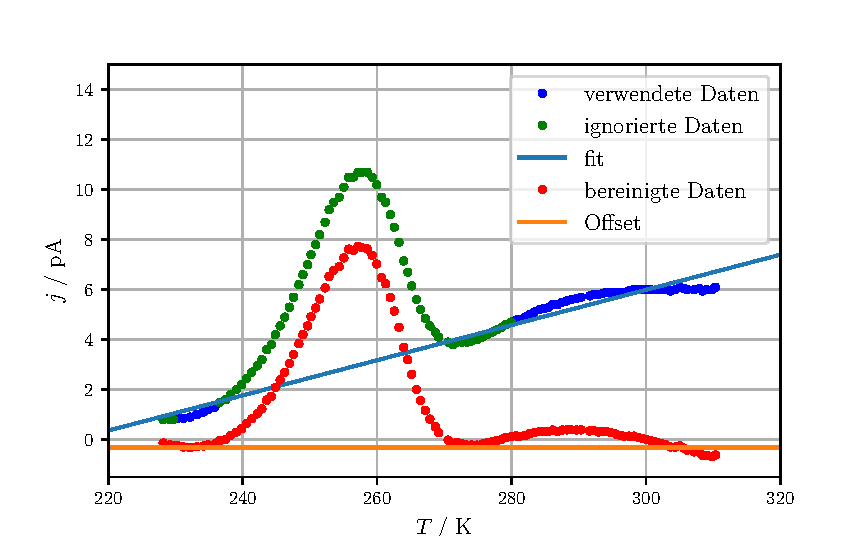
\includegraphics{plot1.pdf}
  \caption{Theoretische Stabilitätsbedingungen für die drei Anordnungen.}
  \label{fig:plot1}
\end{figure}

\FloatBarrier
\subsection{Transversale Moden}
\label{sec:tem}

\subsubsection{$\text{TEM}_{00}$-Mode}

In Tabelle \ref{tab:T00} sind die Messwerte der $\text{TEM}_{00}$-Mode eingetragen und in Abbildung \ref{fig:T00} graphisch dargestellt.
Es wird eine Ausgleichsrechnung der Form
\begin{equation}
  I(r) = a \cdot \exp\left(-2\frac{(r-b)^2}{c^2}\right)
\end{equation}
durchgeführt.
Es ergeben sich die Parameter:
\begin{align*}
a &= \SI{7.04(6)}{\micro\ampere}\\
b &= \SI{3.26(3)}{\milli\metre}\\
c &= \SI{5.92(6)}{\milli\metre}
\end{align*}

 \begin{table}
 	\centering
 	\caption{Die gemessene Stromstärke $I$ entlang der Horizontalen der $\text{TEM}_{\text{00}}$-Mode in Abhängigkeit vom Abstand $r$.}
 	\label{tab:T00}
  \begin{tabular}{c c c c}
    \toprule
    $r$ in mm & $I(r)$ in \si{\micro\ampere} & $r$ in mm & $I(r)$ in \si{\micro\ampere} \\
    \midrule
    12 & 0,1  & 2  & 6,52 \\
    11 & 0,27 & 1  & 5,49 \\
    10 & 0,58 & 0  & 3,81 \\
     9 & 1,08 & -1 & 2,36 \\
     8 & 1,83 & -2 & 1,45 \\
     7 & 3,17 & -3 & 0,76 \\
     6 & 4,7  & -4 & 0,39 \\
     5 & 5,93 & -5 & 0,16 \\
     4 & 6,87 & -6 & 0,05 \\
     3 & 6,75 & & \\
    \bottomrule
  \end{tabular}
 \end{table}

\begin{figure}
  \centering
  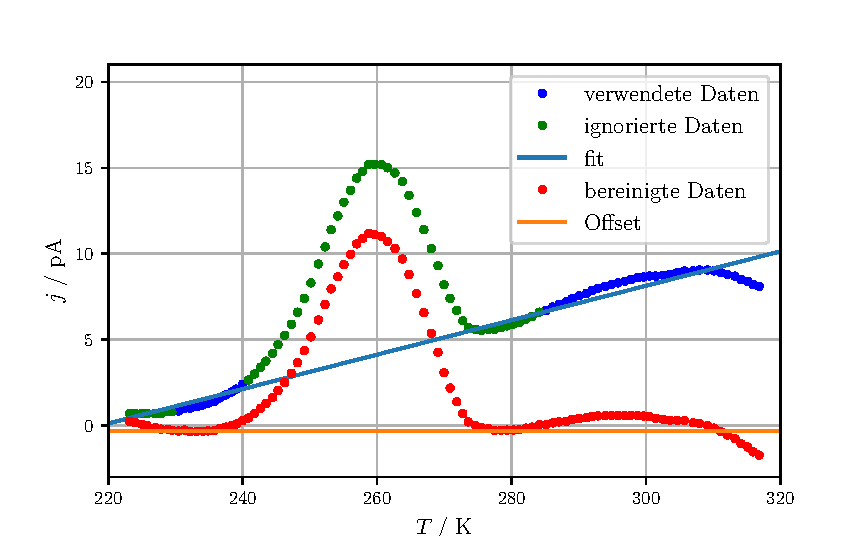
\includegraphics{plot2.pdf}
  \caption{Intensitätsverteilung der $\text{TEM}_{00}$-Mode.}
  \label{fig:T00}
\end{figure}

\subsubsection{$\text{TEM}_{01}$-Mode}

Für die $\text{TEM}_{01}$-Mode wird die Ausgleichsfunktion wie folgt abgewandelt:
\begin{equation}
  I(r) = a \cdot \frac{4(r-b)^2}{c^2} \cdot \exp\left(-2\frac{(r-b)^2}{c^2}\right)
\end{equation}
Die Messdaten sind in Tabelle \ref{tab:T01} aufgelistet.
In Abbildung \ref{fig:T01} ist das Ergebnis der Ausgleichsrechnung zu sehen.
Es ergeben sich die Parameter:
\begin{align*}
a &= \SI{3.21(9)}{\micro\ampere}\\
b &= \SI{3.33(8)}{\milli\metre}\\
c &= \SI{6.25(11)}{\milli\metre}
\end{align*}

\begin{figure}
  \centering
  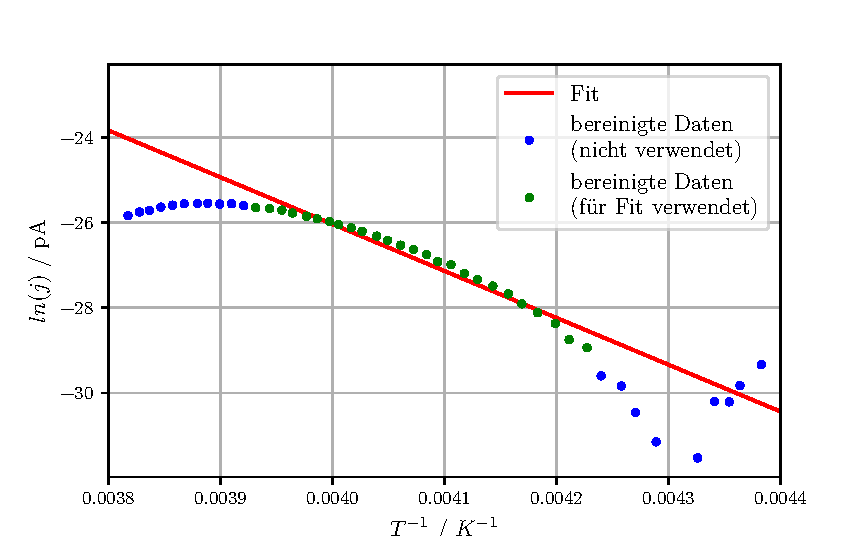
\includegraphics{plot3.pdf}
  \caption{Intensitätsverteilung der $\text{TEM}_{01}$-Mode.}
  \label{fig:T01}
\end{figure}

\begin{table}
 \centering
 \caption{Die gemessene Stromstärke $I$ entlang der Horizontalen der $\text{TEM}_{\text{01}}$-Mode in Abhängigkeit vom Abstand $r$.}
 \label{tab:T01}
 \begin{tabular}{c c c c}
   \toprule
   $r$ in mm & $I(r)$ in \si{\micro\ampere} & $r$ in mm & $I(r)$ in \si{\micro\ampere} \\
   \midrule
   14 & 0,06 & 2  & 0,86 \\
   13 & 0,13 & 1  & 1,45 \\
   12 & 0,39 & 0  & 2,18 \\
   11 & 0,87 & -1 & 2,39 \\
   10 & 1,38 & -2 & 2,54 \\
   9  & 1,72 & -3 & 1,98 \\
   8  & 2,2  & -4 & 1,25 \\
   7  & 2,1  & -5 & 0,7  \\
   6  & 1,45 & -6 & 0,31 \\
   5  & 0,67 & -7 & 0,18 \\
   4  & 0,04 & -8 & 0,1  \\
   3  & 0,21 & -9 & 0,05 \\
   \bottomrule
 \end{tabular}
\end{table}

\subsubsection{$\text{TEM}_{02}$-Mode}

Für die $\text{TEM}_{02}$-Mode wird die Ausgleichsfunktion erneut angepasst:
\begin{equation}
  I(r) = a \cdot \left(\frac{8(r-b)^2}{c^2}-2\right)^2 \cdot \exp\left(-2\frac{(r-b)^2}{c^2}\right)
\end{equation}
Mit den Messdaten aus Tabelle \ref{tab:T02} wird die Ausgleichsrechnung durchgeführt.
Diese liefert die Parameter:
\begin{align*}
a &= \SI{0.069(4)}{\micro\ampere}\\
b &= \SI{2.57(15)}{\milli\metre}\\
c &= \SI{6.46(16)}{\milli\metre}
\end{align*}
In Abbildung \ref{fig:T02} ist das Ergebnis dargestellt.

\begin{figure}
  \centering
  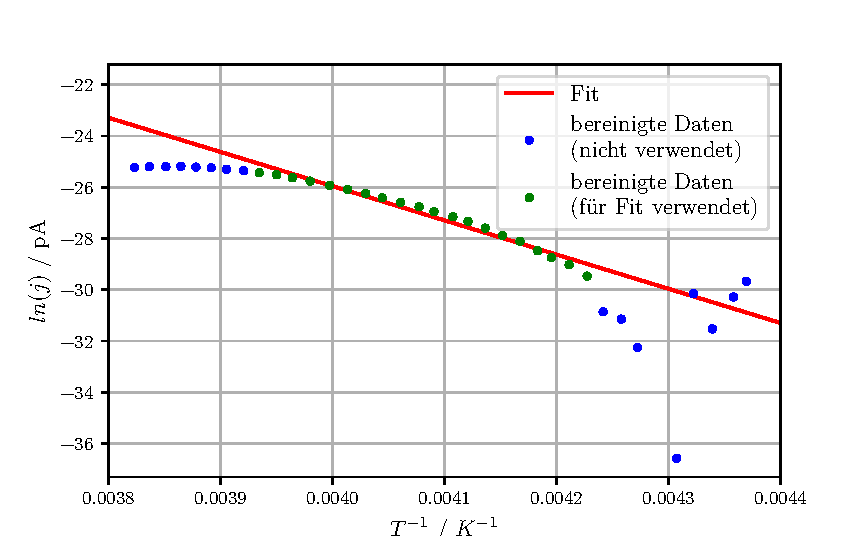
\includegraphics{plot4.pdf}
  \caption{Intensitätsverteilung der $\text{TEM}_{02}$-Mode.}
  \label{fig:T02}
\end{figure}

\begin{table}
 \centering
 \caption{Die gemessene Stromstärke $I$ entlang der Horizontalen der $\text{TEM}_{\text{02}}$-Mode in Abhängigkeit vom Abstand $r$.}
 \label{tab:T02}
 \begin{tabular}{c c c c}
   \toprule
   $r$ in mm & $I(r)$ in \si{\micro\ampere} & $r$ in mm & $I(r)$ in \si{\micro\ampere} \\
   \midrule
   14  & 0,04 & 1   & 0,12 \\
   13  & 0,11 & 0   & 0,04 \\
   12  & 0,16 & -1  & 0,018 \\
   11  & 0,22 & -2  & 0,09 \\
   10  & 0,27 & -3  & 0,35 \\
   9   & 0,25 & -4  & 0,47 \\
   8   & 0,18 & -5  & 0,45 \\
   7   & 0,07 & -6  & 0,36 \\
   6   & 0,01 & -7  & 0,29 \\
   5   & 0,05 & -8  & 0,19 \\
   4   & 0,16 & -9  & 0,09 \\
   3   & 0,21 & -10 & 0,04 \\
   2   & 0,19 & & \\
   \bottomrule
 \end{tabular}
\end{table}

\subsection{Polarisation}
\label{sec:pol}

Es wird die Polarisation des Lasers untersucht.
Dafür wird die Intensität des Lasers bei verschiedenen Polarisationswinkeln gemessen.
Die Werte sind in Tabelle \ref{tab:polarisation} eingetragen und in Abbildung \ref{fig:polarisation} graphisch dargestellt.
Es wird eine Ausgleichsrechnung der Form
\begin{equation}
  I(\varphi) = I_0 \cos^2\left(\varphi+\varphi_0\right)
\end{equation}
durchgeführt.
Diese liefert die Parameter:
\begin{align*}
I_0 &= \SI{149.42(212)}{\micro\ampere}\\
\varphi_0 &= \SI{-78.33(1)}{rad}\\
\end{align*}

\begin{figure}
  \centering
  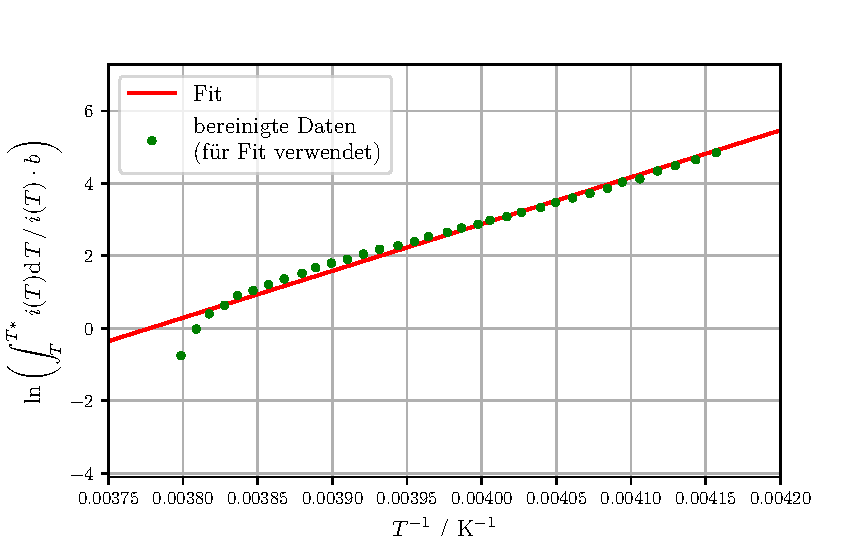
\includegraphics{plot5.pdf}
  \caption{Abhängigkeit der Intensität vom Polarisationswinkel.}
  \label{fig:polarisation}
\end{figure}

\begin{table}
 \centering
 \caption{Polarisationswinkel $\varphi$ und Stromstärke $I$.}
 \label{tab:polarisation}
 \begin{tabular}{c c c c}
   \toprule
   $\varphi$ in Grad & $I(\varphi)$ in \si{\micro\ampere} & $\varphi$ in Grad & $I(\varphi)$ in \si{\micro\ampere} \\
   \midrule
   0  & 138 & 100 & 18  \\
   10 & 126 & 110 & 35  \\
   20 & 104 & 120 & 63  \\
   30 & 80  & 130 & 82  \\
   40 & 59  & 140 & 120 \\
   50 & 32  & 150 & 142 \\
   60 & 14  & 160 & 163 \\
   70 & 3   & 170 & 148 \\
   80 & 0.3 & 180 & 140 \\
   90 & 5   & & \\
   \bottomrule
 \end{tabular}
\end{table}

\subsection{Multimodenuntersuchung}
\label{sec:mul}

Es werden die Frequenzen $f$ der longitudinalen Moden für verschiedene Resonatorlängen vermessen und die mittlere Frequenzdifferenz $\Delta f$ berechnet.
Die Werte sind in Tabelle \ref{tab:longitudinal} eingetragen.
Theoretisch ist folgender Zusammenhang zu erwarten mit der Lichtgeschwindigkeit im Vakuum $c_0$:
\begin{equation}
  \Delta\lambda = \frac{c_0}{\Delta f} = 2L
\end{equation}
Eine Ausgleichsrechnung der Form $\Delta\lambda(L) = a \cdot L$ liefert:
\begin{equation*}
  a = \num{2.016 \pm 0.003}
\end{equation*}
Die Abhängigkeit der Frequenzdifferenzen von der Resonatorlänge ist in Abbildung \ref{fig:longitudinal} dargestellt.

\begin{table}
 \centering
 \caption{Die gemessenen Frequenzen und mittleren Frequenzdifferenzen für verschiedene Resonatorlängen.}
 \label{tab:longitudinal}
 \begin{tabular}{c c c c c c c c}
   \toprule
   $L$ in cm & \multicolumn{6}{c}{Frequenzen $f$ in MHz} & $\Delta f$ in MHz  \\
   \midrule
   87     & 173 & 341 & 510 & 683 & 851 & 1020 & 169 \\
   91     & 165 & 326 & 491 & 653 & 818 & 979  & 163 \\
   96.5   & 158 & 311 & 465 & 619 & 773 & 926  & 154 \\
   105.7  & 143 & 281 & 424 & 563 & 705 & 844  & 140 \\
   114    & 131 & 263 & 394 & 525 & 656 & 784  & 131 \\
   121.3  & 124 & 248 & 371 & 495 & 615 & 739  & 123 \\
   128    & 116 & 233 & 349 & 469 & 585 & 701  & 117 \\
   134    & 113 & 225 & 334 & 446 & 555 & 668  & 111 \\
   \bottomrule
 \end{tabular}
\end{table}

\begin{figure}
  \centering
  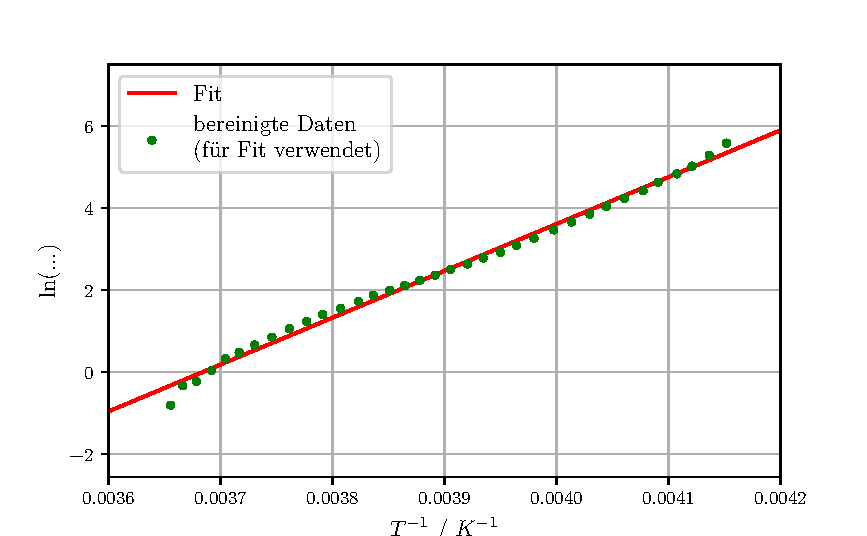
\includegraphics{plot6.pdf}
  \caption{Die gemessenen Differenzen $\Delta\lambda$ in Abhängigkeit der Resonatorlänge $L$.}
  \label{fig:longitudinal}
\end{figure}

Durch den Dopplereffekt kommt es zur Verbreiterung der Spektrallinien.
Dieser Effekt wird Doppler-Verbreiterung genannt und durch die Halbwertsbreite $\delta f$ beschrieben.
\begin{equation}
  \delta f = \frac{f_0}{c} \sqrt{\frac{8 k_b T \ln(2)}{m}}
\end{equation}
Mit der Neonatommasse von $m=20,18$ u, einer Tempetatur von $T = 300$ K und für die rote Linie mit $\lambda = 632,8$ nm beträgt die Halbwertsbreite:
\begin{equation*}
  \delta f \approx \SI{1300}{MHz}
\end{equation*}
Der Laser läuft im Multimodenbetrieb, wenn die Halbwertsbreite $\delta f$ ein Vielfaches der Frequenzabstände $\Delta f$ zwischen den einzelnen Moden ist.

\subsection{Wellenlänge}
\label{sec:wel}

Die Wellenlänge des Lasers kann mithilfe der Formel
\begin{equation}
  \lambda = \frac{\sin\left(\tan\left(\frac{d_n}{L}\right)\right)}{g \cdot n}
\end{equation}
bestimmt werden.
Dabei ist $L$ der Abstand zwischen Gitter und Schirm, $d_n$ der Abstand des n-ten Nebenmaxima vom Hauptmaxima und $g$ die Gitterkosntante.
Die Messwerte und Ergebnisse sind in Tablle \ref{tab:wel} aufgeführt.
Für die Wellenlänge ergibt sich so ein Mittelwert von \SI{631.29(539)}{nm}.

\begin{table}
 \centering
 \caption{Die Ordnung $n$ der Nebenmaxima, ihr Abstand $d_n$ zum Hauptmaximum,  sowie die berechnete Wellenlänge $\lambda$ für verschiedene $L$ und $g$.}
 \label{tab:wel}
 \begin{tabular}{c c c c c}
   \toprule
   Gitterkosntante $g$ & $L$ in cm & Ordnung & Abstand $d_n$ in cm & Wellenlänge $\lambda$ in nm \\
   \midrule
   100 Linien/mm & 88,5 & 1 & 5,55  & 627,53 \\
   & & 1 & 5,6 & 633,19 \\
   80 Linien/mm & 90 & 1 & 4,5  & 625,26 \\
   & & 1 & 4,6 & 639,17\\
   \bottomrule
 \end{tabular}
\end{table}
